
\subsection{The Control Flow graph}\label{abstrCntrFlow}
In this section we discuss how the control flow graph of a bytecode is transformed in an acyclic control flow graph. We assume that the bytecode is provided 
with sufficient specification and in particular loop invariants. Under the assumption for invariant presence we may ``cut'' the control flow graph at every program point
where an invariant must hold and ``place'' at that point the invariant. This needs the introduction of several definitions.

%As we  already stated we assume that loops in method bodies are  \textit{annotated} with appropriate invariants. 
%Related works like in \cite{WildmoserN-ESOP05} use different approach where loop invariants are inferred. Anyways inferring invariants is not decidable. 
%Rather we propose the scheme where the programmer writes the invariants during the program development  
%and on compilation time compiles them in BCL.. Here we describe which are the points in the bytecode which are "cut". This needs the introduction
%of several definitions.
     
 A method body is an array of bytecode instructions that is denoted with $i$ and the $k-th$ instruction
 in the bytecode is  denoted with $i_{k}$.
% We denote by $\Gamma  = ( \Omega, \execRel)$ the control flow graph of abytecode where the set of nodes $\Omega$ is the set of basic blocks of the bytecode.
 We assume that method's bytecode has exactly one entry point(every execution of a method starts at the entry point instruction) and we denote it with $i_{\tt{entry}}$.  Using standard terminology \cite{ARUCom1986}, a
basic block is a code segment that has no unconditional jump or
conditional branch statements except for possibly the last
statement, and none of its statements, except possibly the first,
is a target of any jump or branch statement. 
 We denote a block starting at instruction  $i_{j}$ with $\blockm{j}$.The block starting at the entry instruction is denoted with $\blockm{entry}$.
 The execution relation  $\blockm{j} \execRel \blockm{k}$  states that block $\blockm{k}$ may be executed immediately after $\blockm{j}$ in some execution path of the method. For example if  instruction $\tt{i_{k}}$ = \texttt{athrow} is the last of the block $\blockm{j}$ then 
$\blockm{j} \execRel \blockm{n}$, where  $\blockm{n}$ is the first block of an exception handler that protects $\tt{i_{k}}$ 
% Definition \ref{execRel} states formally the execution relation.
% \begin{defn}[Execution relation between blocks]\label{execRel}
%\begin{tabbing}
%\\Let \=  have \= the block $\blockm{j}$ such that  it ends with instruction \\ 
%$\tt{i_{k}}$ and it is not a return instruction\\
%\>  if $\tt{i_{k}}$ = \texttt{if\_cond n} then   $\blockm{j} \execRel \blockm{n}$ and $\blockm{j} \execRel  \blockm{k+1} $ \\
%\>  if $\tt{i_{k}}$ = \texttt{goto n} then $\blockm{j} \execRel \blockm{n}$ \\
%\>  if $\tt{i_{k}}$ = \texttt{athrow} then $\blockm{j} \execRel \blockm{n}$ for all \texttt{n}, such \\
%\> \> that $\blockm{n}$ is the first\\
%\> \> block of an exception handler that protects $\tt{i_{k}}$ \\
%\>  if $\tt{i_{k}}$ = \texttt{jsr n} then $\blockm{j} \execRel \blockm{n}$ \\
%\>  if  $\tt{i_{k}}$ = \texttt{ret n} then  $ \blockm{j} \execRel \blockm{s}$\\
%\> \> for all s that are indexes of instruction following \\
%\> \> a \texttt{jsr} to the subroutine that ends with $\tt{i_{k}}$ instruction\\
%\>  else $\blockm{j}  \execRel   \blockm{k+1}$
%\end{tabbing}
%\end{defn}

%We say that there exists a path between $\blockm{i}$ and $\blockm{j}$ and we note it with  $\pathm{i}{j}$, if there exists blocks 
%$\blockm{s_{1}}... \blockm{s_{n}}$ such that $\blockm{i} \execRel \blockm{s_{1}} \execRel \blockm{s_{2}}... \blockm{s_{n}} \execRel  \blockm{j}$

\begin{defn}[Loop Definition]
\label{defLoop}
Let's have a bytecode program. We say that $\blockm{s}$ is the entry block of loop $l$ in $\Pi$ and $\blockm{e}$ is the end block of $l$ if:
\begin{itemize}
\item every path in the control flow graph starting at the entry block $\blockm{entry}$ of $\Pi$ and that reaches $\blockm{e}$, passes through  $\blockm{s}$ 
  i.e.$ \blockm{entry} \execRel^{*}  \blockm{s} \execRel^{*} \blockm{e}$
\item $\blockm{e} \execRel \blockm{s}$
\end{itemize}
\end{defn}
%\subsection{Acyclic control flow graph} \label{graph}
We abstract the execution relation $\execRel$ to the acyclic execution relation $\execRel^A$ as follows. 
%We consider the acyclic graph $\Gamma^A = ( \Omega, \execRel^A)$ obtained from the control flow graph 
%$\Gamma  = ( \Omega, \execRel)$ of a well formed bytecode $ \Pi $ where the relation $\execRel^A$ is a subset of the  execution relation $\execRel$.

\begin{defn}[Acyclic Execution relation]
\label{acyclicExRel}
Let's have a bytecode and let's have in it the two basic blocks  $\blockm{i} $ and   $\blockm{j}$. We say 
that $\blockm{i} \execRel^A \blockm{j}$ iff
\begin{itemize}
\item $\blockm{i} \execRel \blockm{j}$
\item and block $\blockm{i}$ and block $\blockm{j}$ are not the end and the entry blocks respectively of the same loop, see loop definition~\ref{defLoop}.
\end{itemize}
\end{defn}

We give at fig.~\ref{blockBC} the control flow graph of the method replace given earlier in fig.~\ref{replaceSrc}. The figure shows that the acyclic relation
excludes edges between loop entry and loop end blocks and that at that place the corresponding loop invariant must hold.  

\begin{figure}[p]
\begin{center}
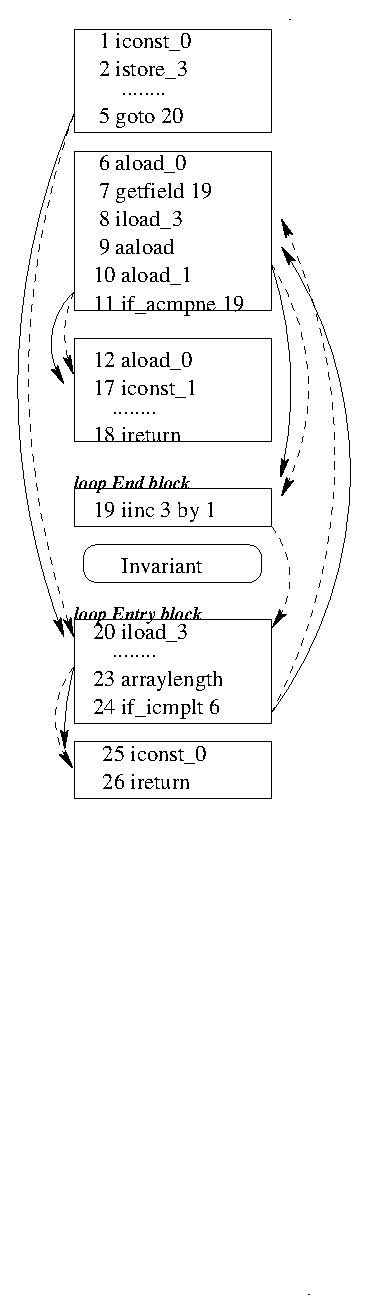
\epsfig{file=graph1.eps}
\end{center}
dashed arrows stand for the standard execution relation \\ 
black arrows represent the acyclic execution relation \\
bytecode basic blocks are placed in boxes \\
the invariant is placed between the blocks where it must hold
\caption{control flow graph of method \texttt{replace} from fig. ~\ref{replaceSrc} }
\label{blockBC}
\end{figure}

%Now a path in $\Gamma^A$  is a list of blocks between which is established a relation $\execRel^A$ and that starts at the entry point instruction and whose last block is a block that does not have next block.

